% pdflatex nn-times-gpu.tex && rm *.aux *.log
% pdftoppm nn-times-gpu.pdf -rx 500 -ry 500 nn-times-gpu -png

\documentclass[varwidth]{standalone}
\usepackage{pgfplots}
\usepackage{graphicx}
\begin{document}

\resizebox{0.95\columnwidth}{!} {
% BIRD
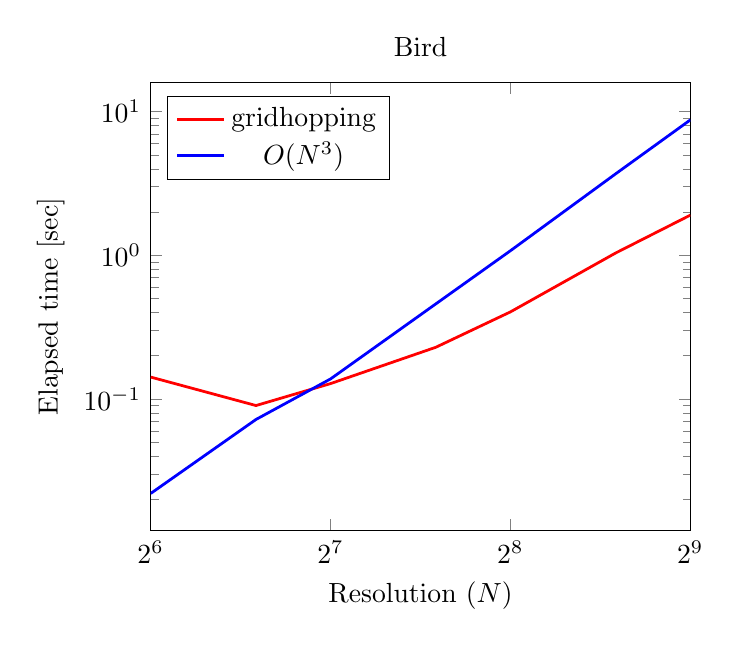
\begin{tikzpicture}
\begin{axis} [
	title=Bird,
	ymode=log,
	xlabel={Resolution ($N$)},
	ylabel={Elapsed time [sec]},
	xmin=64, xmax=512,
	xmode=log, log basis x=2,
	legend pos=north west
]
		\addplot[color=red, line width=1]
			coordinates {
				(64.000000, 0.142000)(96.000000, 0.090000)(128.000000, 0.128000)(192.000000, 0.229000)(256.000000, 0.404000)(384.000000, 1.038000)(512.000000, 1.905000)
			};
		\addplot[color=blue, line width=1]
			coordinates {
				(64.000000, 0.022000)(96.000000, 0.072000)(128.000000, 0.138000)(192.000000, 0.459000)(256.000000, 1.077000)(384.000000, 3.693000)(512.000000, 8.765000)
			};
		\legend{gridhopping,$O(N^3)$}
\end{axis}
\end{tikzpicture}
% FROG
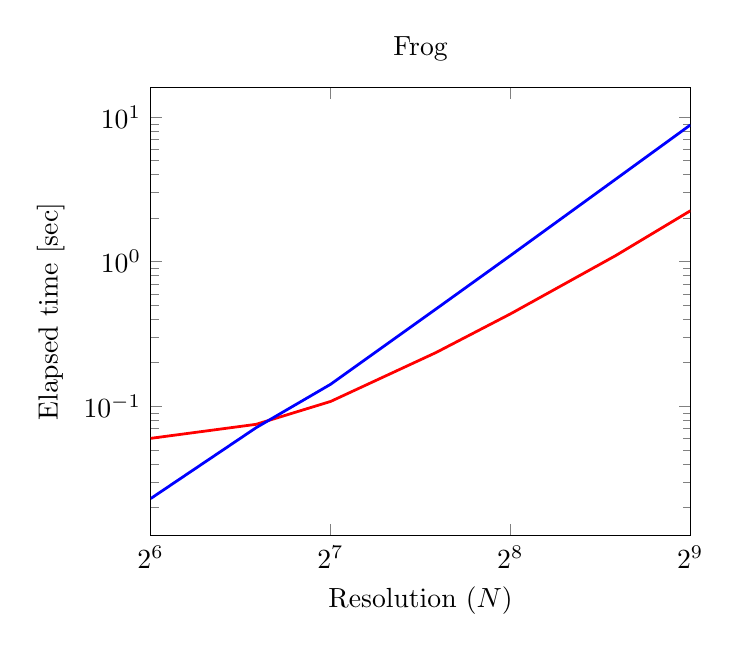
\begin{tikzpicture}
\begin{axis} [
	title=Frog,
	ymode=log,
	xlabel={Resolution ($N$)},
	ylabel={Elapsed time [sec]},
	xmin=64, xmax=512,
	xmode=log, log basis x=2,
	legend pos=north west
]
		\addplot[color=red, line width=1]
			coordinates {
				(64.000000, 0.060000)(96.000000, 0.075000)(128.000000, 0.108000)(192.000000, 0.235000)(256.000000, 0.436000)(384.000000, 1.103000)(512.000000, 2.253000)
			};
		\addplot[color=blue, line width=1]
			coordinates {
				(64.000000, 0.023000)(96.000000, 0.071000)(128.000000, 0.142000)(192.000000, 0.470000)(256.000000, 1.105000)(384.000000, 3.726000)(512.000000, 8.842000)
			};
\end{axis}
\end{tikzpicture}
% CATS
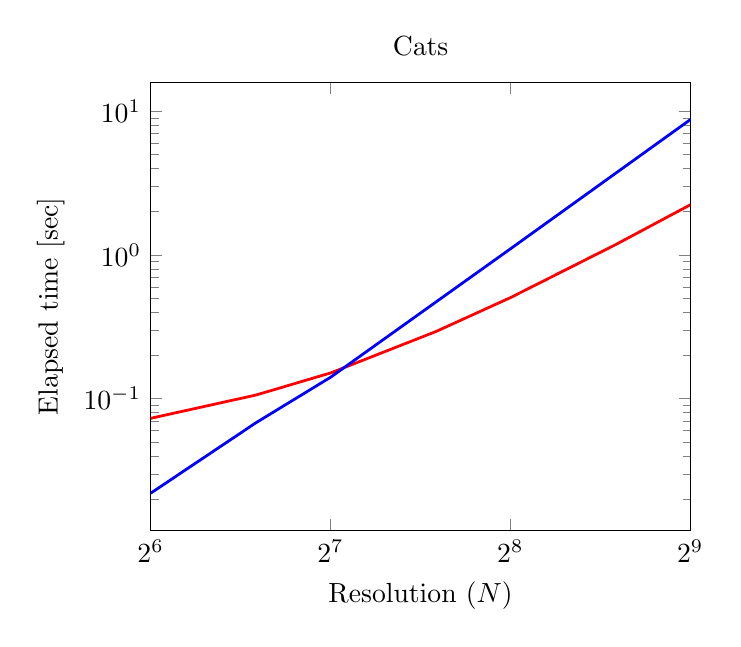
\begin{tikzpicture}
\begin{axis} [
	title=Cats,
	ymode=log,
	xlabel={Resolution ($N$)},
	ylabel={Elapsed time [sec]},
	xmin=64, xmax=512,
	xmode=log, log basis x=2,
	legend pos=north west
]
		\addplot[color=red, line width=1]
			coordinates {
				(64.000000, 0.073000)(96.000000, 0.106000)(128.000000, 0.151000)(192.000000, 0.293000)(256.000000, 0.505000)(384.000000, 1.181000)(512.000000, 2.235000)
			};
		\addplot[color=blue, line width=1]
			coordinates {
				(64.000000, 0.022000)(96.000000, 0.068000)(128.000000, 0.141000)(192.000000, 0.470000)(256.000000, 1.104000)(384.000000, 3.706000)(512.000000, 8.756000)
			};
\end{axis}
\end{tikzpicture}
}
\\
\resizebox{0.95\columnwidth}{!} {
% BUNNY
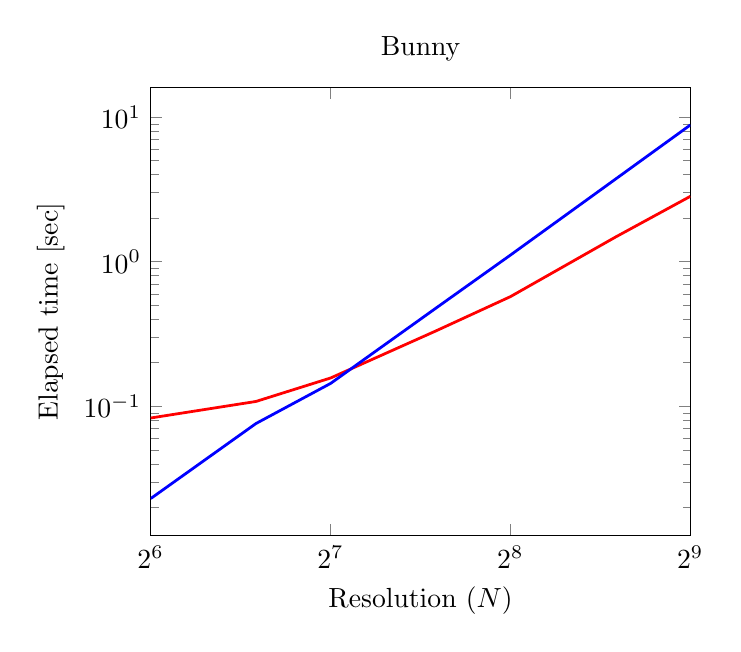
\begin{tikzpicture}
\begin{axis} [
	title=Bunny,
	ymode=log,
	xlabel={Resolution ($N$)},
	ylabel={Elapsed time [sec]},
	xmin=64, xmax=512,
	xmode=log, log basis x=2,
	legend pos=north west
]
		\addplot[color=red, line width=1]
			coordinates {
				(64.000000, 0.083000)(96.000000, 0.108000)(128.000000, 0.157000)(192.000000, 0.332000)(256.000000, 0.574000)(384.000000, 1.484000)(512.000000, 2.836000)
			};
		\addplot[color=blue, line width=1]
			coordinates {
				(64.000000, 0.023000)(96.000000, 0.076000)(128.000000, 0.144000)(192.000000, 0.477000)(256.000000, 1.113000)(384.000000, 3.738000)(512.000000, 8.840000)
			};
\end{axis}
\end{tikzpicture}
% MUSHROOMS
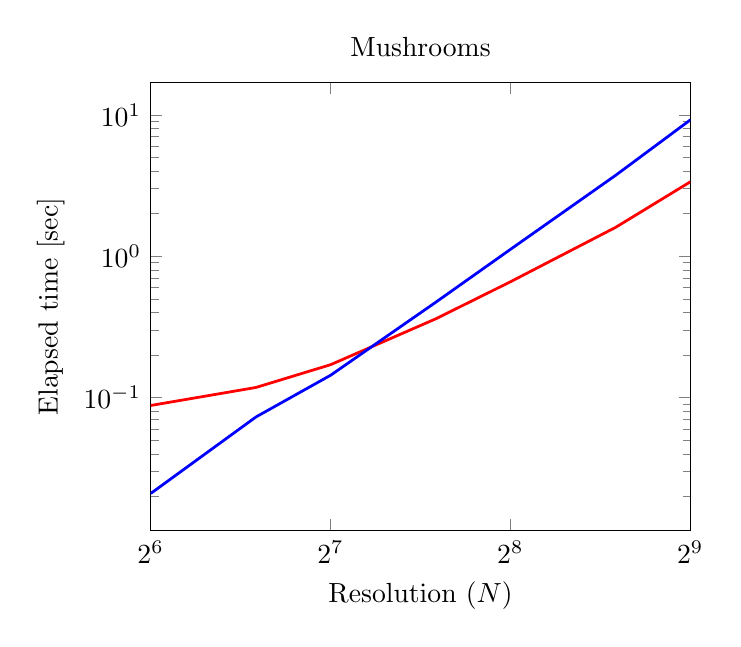
\begin{tikzpicture}
\begin{axis} [
	title=Mushrooms,
	ymode=log,
	xlabel={Resolution ($N$)},
	ylabel={Elapsed time [sec]},
	xmin=64, xmax=512,
	xmode=log, log basis x=2,
	legend pos=north west
]
		\addplot[color=red, line width=1]
			coordinates {
				(64.000000, 0.088000)(96.000000, 0.118000)(128.000000, 0.171000)(192.000000, 0.361000)(256.000000, 0.660000)(384.000000, 1.601000)(512.000000, 3.361000)
			};
		\addplot[color=blue, line width=1]
			coordinates {
				(64.000000, 0.021000)(96.000000, 0.073000)(128.000000, 0.144000)(192.000000, 0.473000)(256.000000, 1.119000)(384.000000, 3.737000)(512.000000, 9.211000)
			};
\end{axis}
\end{tikzpicture}
% WHALE
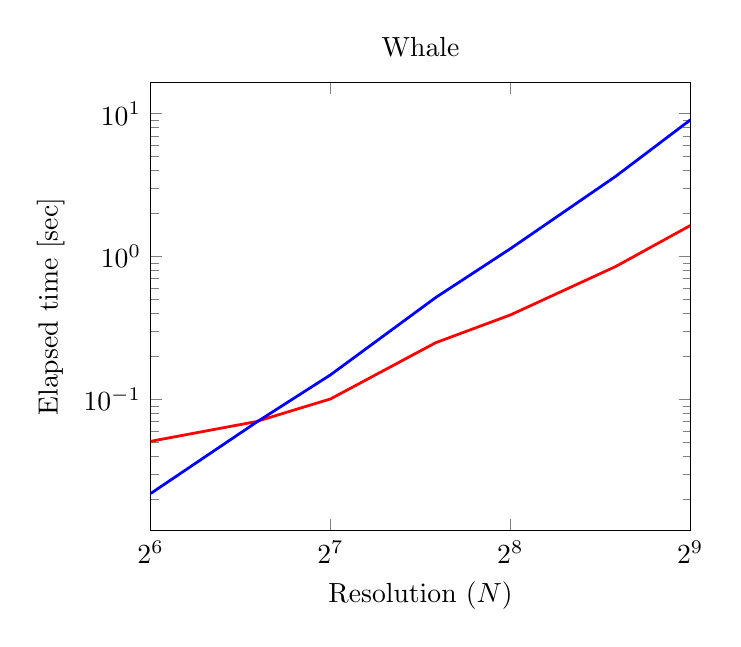
\begin{tikzpicture}
\begin{axis} [
	title=Whale,
	ymode=log,
	xlabel={Resolution ($N$)},
	ylabel={Elapsed time [sec]},
	xmin=64, xmax=512,
	xmode=log, log basis x=2,
	legend pos=north west
]
		\addplot[color=red, line width=1]
			coordinates {
				(64.000000, 0.051000)(96.000000, 0.070000)(128.000000, 0.101000)(192.000000, 0.250000)(256.000000, 0.391000)(384.000000, 0.853000)(512.000000, 1.652000)
			};
		\addplot[color=blue, line width=1]
			coordinates {
				(64.000000, 0.022000)(96.000000, 0.069000)(128.000000, 0.149000)(192.000000, 0.518000)(256.000000, 1.138000)(384.000000, 3.649000)(512.000000, 9.065000)
			};
\end{axis}
\end{tikzpicture}
}

\end{document}
